\item A montagem tem uma massa de \SI{5}{\kilogram} e raio de giração $k_{G}=\SI{.18}{\meter}$ em relação a seu centro de massa $G$. A energia cinética da montagem é \SI{46.5}{\newton\cdot\meter} quando ela está na posição mostrada. Se ela rola no sentido anti-horário sobre a superfície sem deslizar, determine sua quantidade de movimento linear nesse instante.

\import{../answers}{answer-1}

\vspace{-.8cm}
\begin{flushright}
	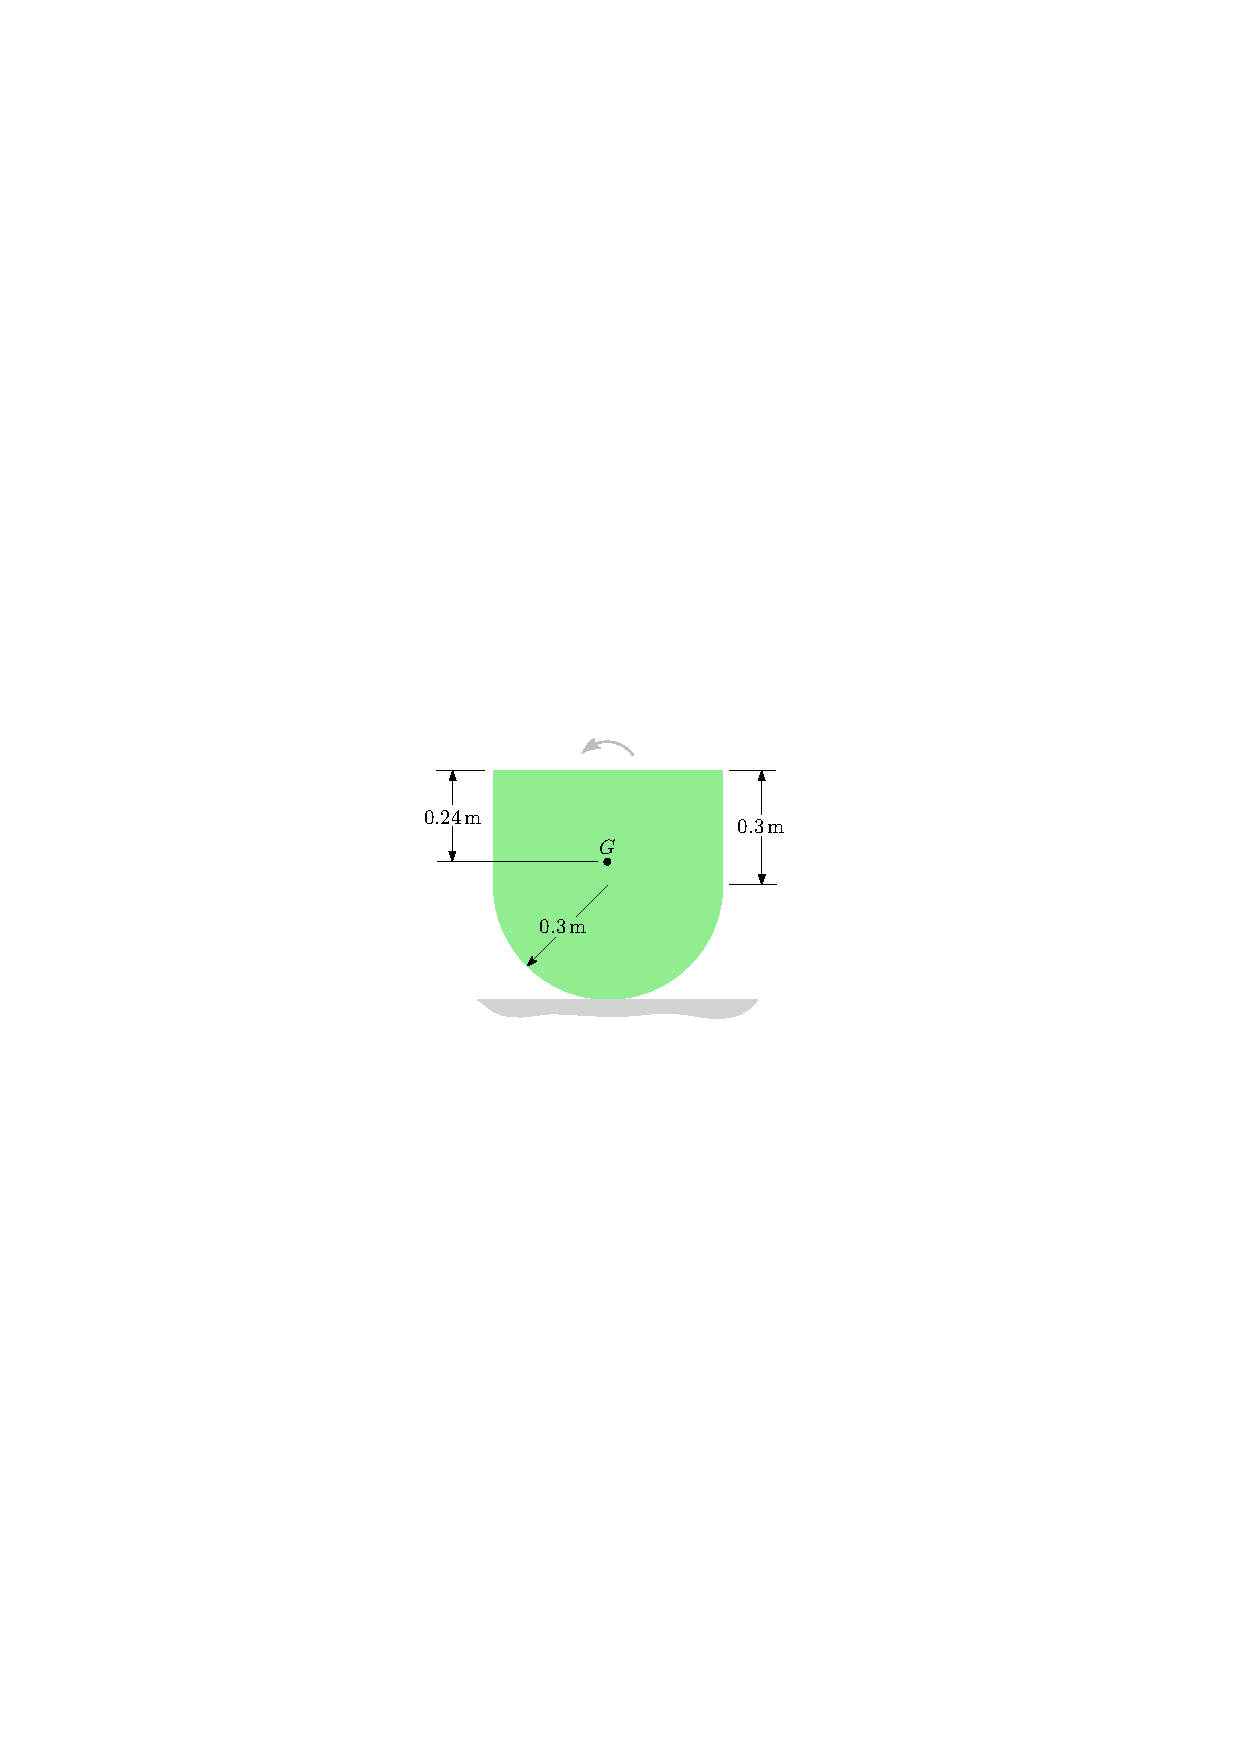
\includegraphics[scale=1.2]{../../images/draw_0_9}
\end{flushright}